\section{Discussion and Analysis}
\label{sec:discussion}

\quad In this section we discuss the implementation details of the HBlast architecture on FPGA. Detailed reconfiguration performance numbers are reported. 

\subsection{Implementation}
\quad Xilinx ISE was used for implementation. The proposed platform was implemented and hardware validated on a Xilinx VC709 evaluation board containing a Virtex-7 XC7VX690T-2FFG1761C FPGA. The static and reconfigurable regions on the FPGA are shown in \textit{Fig.\ref{fig:regions}}. 
\\
\subsection{Resource utilization}
Resource utilization is shown in \textit{Table \ref{tab:util}}. On the Virtex-7 FPGA the platform consumes about \% of logic and BRAM utilization is about \%.

\begin{table}[!t]
\caption {Table Title} \label{tab:util}
\begin{tabular}{l|l|l|l}
\hline
FPGA module        & Slice LUTs & Slice Regs & Block RAM Tile \\ \hline
HBlast             & 11430      & 10738      & 1              \\
bridge             & 68         & 641        & 0              \\
memoryInt          & 5321       & 4809       & 0              \\
Expand             & 2342       & 2410       & 0              \\
hitMem             & 2958       & 808        & 0              \\
queryB             & 39         & 612        & 0              \\
u\_mig\_7series\_0 & 6002       & 4676       & 1              \\ \hline

\end{tabular}
\end{table}

\begin{table}[]
\begin{center}
\caption {Table Title} \label{tab:util2}
\begin{tabular}{|l|l|l|l|}
\hline
Resource & Estimation & Available & Utiliztion \% \\ \hline
LUT      & 5428       & 433200    & 1.25          \\
FF       & 6062       & 866400    & 0.70          \\
IO       & 104        & 850       & 12.24         \\ \hline
\end{tabular}
\end{center}
\end{table}



\subsection{Timing analysis}

In VC709 board system clock is 200MHz generated by frequency oscillator. Therefore, there is no slack  the maximum frequency will be same as the oscillators frequency. \textit{Table \ref{tab:timingSlack}} shows the timing report of our design. 


\begin{table}[]
\begin{center}
\caption {Table Title} \label{tab:timingSlack}
\scalebox{0.85}{%
\begin{tabular}{|l|l|l|l|}
\hline
Total slack, ns & Required time, ns & Arrival time, ns & Maximum frequency, MHz \\ \hline
-0.76           & 5.000             & 5.76           & 173.6                  \\ \hline
\end{tabular}}
\end{center}
\end{table}





\begin{table}[]
\begin{tabular}{ccclc} 
\hline
\multicolumn{1}{|c|}{\begin{tabular}[c]{@{}c@{}}Calibaration\\ complete, ns\end{tabular}} & \multicolumn{1}{c|}{\begin{tabular}[c]{@{}c@{}}Query\\ valid, ns\end{tabular}} & \multicolumn{1}{c|}{\begin{tabular}[c]{@{}c@{}}Read data\\ valid,ns\end{tabular}} & \multicolumn{1}{c|}{\begin{tabular}[c]{@{}c@{}}Process\\ End,ns\end{tabular}} & \multicolumn{1}{c|}{\begin{tabular}[c]{@{}c@{}}Query and data\\ match on database, \\ nth  512 bit\end{tabular}} \\ \hline
\multicolumn{1}{|c|}{53600}                                                               & \multicolumn{1}{c|}{60994}                                                     & \multicolumn{1}{c|}{61169}                                                        & \multicolumn{1}{l|}{xxxxx}                                                    & \multicolumn{1}{c|}{1st}                                                                                         \\ \hline
\multicolumn{1}{|c|}{53600}                                                               & \multicolumn{1}{c|}{60994}                                                     & \multicolumn{1}{c|}{61169}                                                        & \multicolumn{1}{c|}{yyyy}                                                     & \multicolumn{1}{c|}{4th}                                                                                         \\ \hline
\multicolumn{1}{l}{}                                                                      & \multicolumn{1}{l}{}                                                           & \multicolumn{1}{l}{}                                                              &                                                                               & \multicolumn{1}{l}{}                                                                                            
\end{tabular} \label{tab:timingLatency}
\end{table}


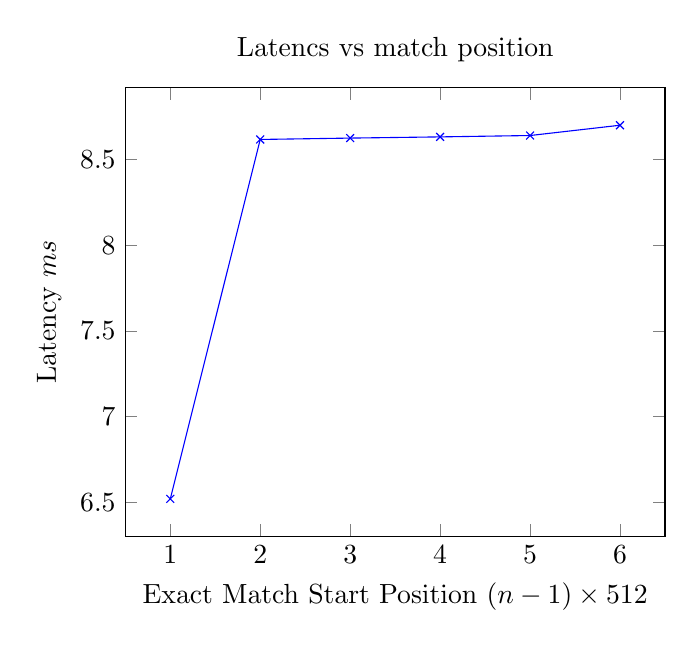
\begin{tikzpicture}
	\begin{axis}[
		xlabel=Exact Match Start Position $(n-1)\times 512$,
		ylabel=Latency $ms$,
		title=Latencs vs match position]
	\addplot[color=blue,mark=x] coordinates {
		(1,6.52)
		(2,8.617)
		(3,8.625)
		(4,8.632)
		(5,8.64)
		(6,8.70)
	};
	\end{axis}
\end{tikzpicture}


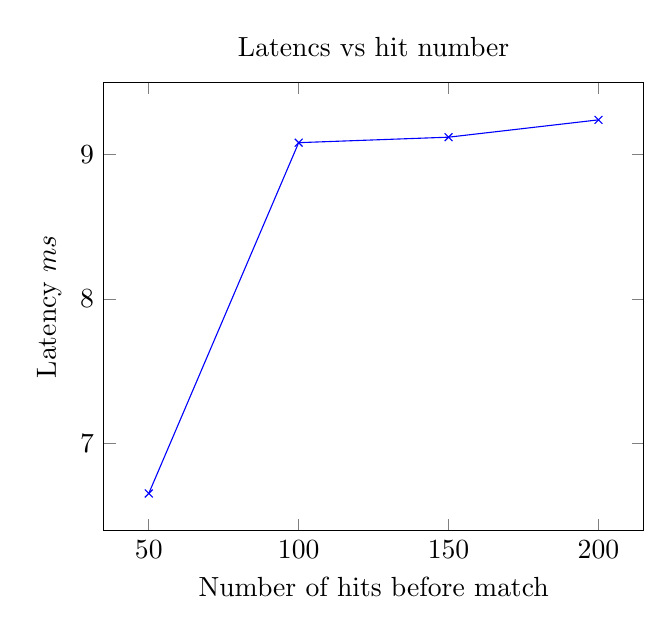
\begin{tikzpicture}
	\begin{axis}[
		xlabel=Number of hits before match,
		ylabel=Latency $ms$,
		title=Latencs vs hit number]
	\addplot[color=blue,mark=x] coordinates {
		(50,6.652)
		(100,9.082)
		(150,9.12)
		(200,9.24)
	};
	\end{axis}
\end{tikzpicture}
